\chapter{Turbostratic carbons II: Impregnation methods}
\label{ch:impregnation}

\newpage
\section*{Abstract}
In recent years, various researchers have investigated alternative methods of introduction of oxidative chemical \gls{porogen} to precursor in the synthesis of \glspl{activated carbon}. These differ from the standard physical mixing method in that they attempt to increase the homogeneity of the precursor-\gls{porogen} mixture while simultaneously decreasing distances between \gls{porogen} and precursor atoms. These techniques include solution impregnation and the carbonisation of organic salts. Such techniques are collectively termed as impregnation techniques for the purposes of this chapter, and have been shown to yield more precise control over pore size, geometry, and pore network connectivity as well as showing promise in facilitation development of improved microporosity.

What is lacking in these studies is insight into the effect of the relative quantity of impregnated \gls{porogen} as well as activation temperature on the pore structure and elemental composition of the derived porous carbons. Thus, this chapter reports the investigation of these variables by two means, (i) hydrothermal impregnation of \ce{KOH} into \acrfull{sd} followed by pyrolysis, and (ii) carbonisation of \acrfull{nc} at varying degrees of substitution. It was found that in the case of the \acrshort{sd}-derived materials, \ce{C} content is drastically improved by this technique relative to more `traditional' methods. In addition at a \ce{KOH}:\acrshort{sd} ratio of \num{2.00}, a carbon with unusually low bulk density (\qty{\sim0.031}{\gram\per\cm\cubed}),  and high mesoporosity (\qty{73}{\percent} by surface area) is produced. As for \acrshort{nc}-derived carbons, in many cases a two-phase highly oxygen-rich product was produced. These properties appear to be a function of both the amount of \ce{Na} in the precursor, as well as activation temperature. Network connectivity and/or pore geometry in the carbons also appears to be a result of these two variables. This work provides scope for investigation of the pore formation mechanisms of these highly unusual carbons.

\newpage

\section[Hydrothermal Sawdust KOH-impregnation]{Hydrothermal Sawdust \ce{KOH}-impregnation}
\label{ss:sd_results}

Eleven SH\textit{x.xx-HHH} samples were produced from the sawdust precursor. In the case of \textit{x.xx} \num{>0.00}, removal of \ce{K} salts \textit{via} washing resulted in the sole product being small amounts of flakey carbonaceous matter that was difficult to isolate as an intermediate. As a result, compositional and porosimetric analysis was difficult to achieve. Furthermore, extensive washing appears to remove extremely fine particles which may have some function in the subsequent pyrolysis step. The three \glspl{hydrochar}, SH0.00-\textit{HHH} were much easier to isolate and analyse. The eleven \glspl{turbostratic carbon} (SA\textit{x.xx-HHH}) were the typical black powders, however SA2.00-250 was very diffuse and clearly has a much lower density relative to the other samples and indeed to that of typical activated/\glspl{turbostratic carbon}.

\subsection{Composition}

CHN elemental microanalysis was used to determine the composition of sawdust precursor and derived carbons; results are show in table \ref{tb:sa_chn}. \acrshort{tga} shows that all samples are fully carbonaceous, i.e. there are no residual \ce{K} compounds present after washing - see appendix, figure \ref{fig:SD_tga}. Thus, in the CHN analysis, the remainder of the sum of \ce{C}, \ce{H} and \ce{N} gravimetric concentrations is assumed to be made up by \ce{O} in table \ref{tb:sa_chn}. In addition, for all carbons there is a single burn-off event at \qty{600}{\degreeCelsius}, as reported previously both for carbons prepared directly from sawdust or from sawdust-derived \gls{hydrochar}.\citep{Balahmar2017Biomass} Therefore, the thermal stability of carbons derived from sawdust does not seem to be significantly affected by the quantity (or even presence) of \ce{KOH} as a \gls{porogen}, the method of preparing the precursor, or the method of introducing \ce{KOH} to the precursor.

\begin{table}[ht!]
    \caption{Composition of SA\textit{x.xx-TTT} carbons according to elemental microanalysis. \ce{O} content is the remaining \unit{\wtpercent} after consideration of the \ce{C}, \ce{H}, and \ce{N}.}
    \label{tb:sa_chn}
    \begin{tabularx}{\textwidth}{lXXXXXX}
    \toprule
        \textbf{Sample} & \multicolumn{4}{c}{\textbf{Concentration / \unit[detect-weight]{\wtpercent}}} & \multicolumn{2}{c}{\textbf{Atomic ratio}} \\
        & \textbf{C} & \textbf{H} & \textbf{N} & \textbf{O} & \textbf{O/C} & \textbf{H/C} \\
    \midrule
        \textbf{\acrshort{sd}} & 45 & 6 & 1 & 48 & 0.80 & 1.62 \\
        \\
        \textbf{SA0.00-200} & 87 & 1.4 & 1.7 & 11 & 0.09 & 0.19 \\
        \textbf{SA0.50-200} & 88 & 0.44 & 0.03 & 12 & 0.10 & 0.06 \\
        \textbf{SA1.00-200} & 90 & 0.15 & 0.94 & 8.8 & 0.07 & 0.02 \\
        \\
        \textbf{SA0.00-250} & 85 & 0.94 & 0.33 & 14 & 0.12 & 0.13 \\
        \textbf{SA0.25-250} & 87 & 0.04 & 0.05 & 13 & 0.12 & 0.13 \\
        \textbf{SA0.50-250} & 93 & 0.00 & 0.52 & 6.2 & 0.05 & - \\
        \textbf{SA1.00-250} & 90 & 0.00 & 0.00 & 9.6 & 0.08 & - \\
        \textbf{SA2.00-250} & 93 & 0.00 & 0.00 & 7.5 & 0.06 & - \\
        \\
        \textbf{SA0.00-300} & 86 & 0.89 & 0.55 & 12 & 0.11 & 0.12 \\
        \textbf{SA0.50-300} & 91 & 0.09 & 0.15 & 8.6 & 0.07 & 0.01 \\
        \textbf{SA1.00-300} & 92 & 0.14 & 0.00 & 7.4 & 0.06 & 0.02 \\
    \bottomrule
    \end{tabularx}
\end{table}

The elemental composition of the sawdust is similar to that previously reported by the Mokaya group.\citep{Balahmar2019Pre, Balahmar2017Biomass} Carbons derived from the slurries formed \textit{via} \gls{htc} at \qtylist[list-units=single, list-final-separator={or }]{250;300}{\degreeCelsius} without the use of \ce{KOH} have slightly lower \ce{C} contents than their \ce{KOH}-activated counterparts, and retained some \ce{H} and \ce{N}. On the other hand, \ce{KOH}-activated samples with \ce{KOH}:\acrshort{sd} mass ratio \num{>0.25} are at least \qty{90}{\percent} carbon with the heteroatoms - excluding \ce{O} - almost completely removed. On the other hand, SA0.00-200 has a very similar \ce{O}/\ce{C} atomic ratio to SA0.50-200. This indicates that at some \gls{htc} temperature between \qtylist[list-units=single]{200;250}{\degreeCelsius}, \ce{KOH} facilitates the breakdown of \ce{O}-rich moieties in the sawdust, resulting in their removal during the activation step. Further, the addition of \ce{KOH} only significantly facilitates this degradation once \ce{KOH}:\ce{C} mass ratio is greater than 0.25. The \ce{O}/\ce{C} atomic ratios of the SA\textit{x.xx}-250 ($x.xx>0.00$) carbons are  lower than those of previously reported carbons derived by the sequential \gls{htc} at \qty{250}{\degreeCelsius} and activation with \ce{KOH} at \qty{800}{\degreeCelsius}. In their report, Balahmar and Mokaya find that the the lowest \ce{O}/\ce{C} (\num{0.12}) was achieved at a \ce{KOH}:\gls{hydrochar} mass ratio of \num{4}.\citep{Balahmar2017Biomass} Thus, the inclusion of \ce{KOH} in the \gls{htc} step provides for a route to a more carbon-rich material, without necessitating the use of higher quantities of \ce{KOH}.

\subsection{Porosity}

It was initially attempted to produce porous carbons \textit{via} \gls{htc} with a \ce{KOH} solution, i.e. without \gls{pyrolysis}. Unsurprisingly this proved ineffective as \gls{activation} typically requires temperatures in excess of \qty{400}{\degreeCelsius}.\citep{Sevilla2014Energy, Blankenship2022Modulating} $A_{BET}$ of these samples (i.e. SH\textit{x.xx-HHH}) was not in excess of \qty{10}{\metre\squared\per\gram}. As for the pyrolised samples, porosity was reasonable, with $A_{BET}$ of least \qty{300}{\metre\squared\per\gram} for samples synthesised without \ce{KOH}, and above \qty{990}{\metre\squared\per\gram} for the \ce{KOH}-activated samples. Full textural characteristics are shown in table \ref{tb:sa_porosity}, as well as the isotherms from which they are derived and \acrshortpl{psd} in figure \ref{fig:SA_n2_isotherms}.\footnote{Individual \glspl{psd} and the kernel fits they are derived from can be found in the appendix, figures \ref{fig:SAxxx-200_isopsd}-\ref{fig:SAxxx-300_isopsd}.} 

\begin{table}[t!]
    \centering
    \caption{Porosity of SA\textit{x.xx-TTT} carbons. $A_{BET}$ derived using the Rouquerol method, the total pore volume, $V_t$ is taken using the single point method. Values in brackets indicate the microporous portion of $A_{BET}$ and $V_t$, calculated using t-plot. Peak pore width, $w_{peak}$ is the maximum of the \acrshort{psd} determined using \acrshort{nldft}, as shown in figure \ref{fig:SA_n2_isotherms}.}
    \label{tb:sa_porosity}
    \begin{tabularx}{0.9\textwidth}{lllllll}
    \toprule
        \textbf{Sample} & \multicolumn{2}{l}{$\mathbf{A_{BET}}$ \textbf{/ \unit[detect-weight]{\metre\squared\per\gram}}}  & \multicolumn{2}{l}{$\mathbf{V_t}$ \textbf{/ \unit[detect-weight]{\cm\cubed\per\gram}}} & \multicolumn{2}{l}{$\mathbf{w_{peak}}$ \textbf{/ \unit{\angstrom}}} \\
    \midrule
        \textbf{SA0.00-200} & 339 & (311, 92\%) & 0.14 & (0.12, 85\%) & 8 \\
        \textbf{SA0.50-200} & 1174 & (1092, 93\%) & 0.47 & (0.42, 89\%) & 7 \\
        \textbf{SA1.00-200} & 1524 & (1398, 92\%) & 0.61 & (0.54, 89\%) & 7 \\
        \\
        \textbf{SA0.00-250} & 452 & (418, 92\%) & 0.18 & (0.16, 89\%) & 6 \\
        \textbf{SA0.25-250} & 994 & (922, 93\%) & 0.39 & (0.35, 90\%) & 6 \\
        \textbf{SA0.50-250} & 1319 & (1242, 94\%) & 0.51 & (0.47, 92\%) & 6 \\
        \textbf{SA1.00-250} & 1341 & (1238, 92\%) & 0.53 & (0.48, 91\%) & 6 \\
        \textbf{SA2.00-250} & 2396 & (644, 27\%) & 0.84 & (0.27, 32\%) & 8 \\
        \\
        \textbf{SA0.00-300} & 323 & (294, 91\%) & 0.13 & (0.11, 85\%) & 9 \\
        \textbf{SA0.50-300} & 1084 & (989, 91\%) & 0.44 & (0.38, 86\%) & 6 \\
        \textbf{SA1.00-300} & 1295 & (1140, 88\%) & 0.54 & (0.44, 82\%) & 6 \\
    \bottomrule
    \end{tabularx}
\end{table}

\begin{figure}[ht!]
    \centering
    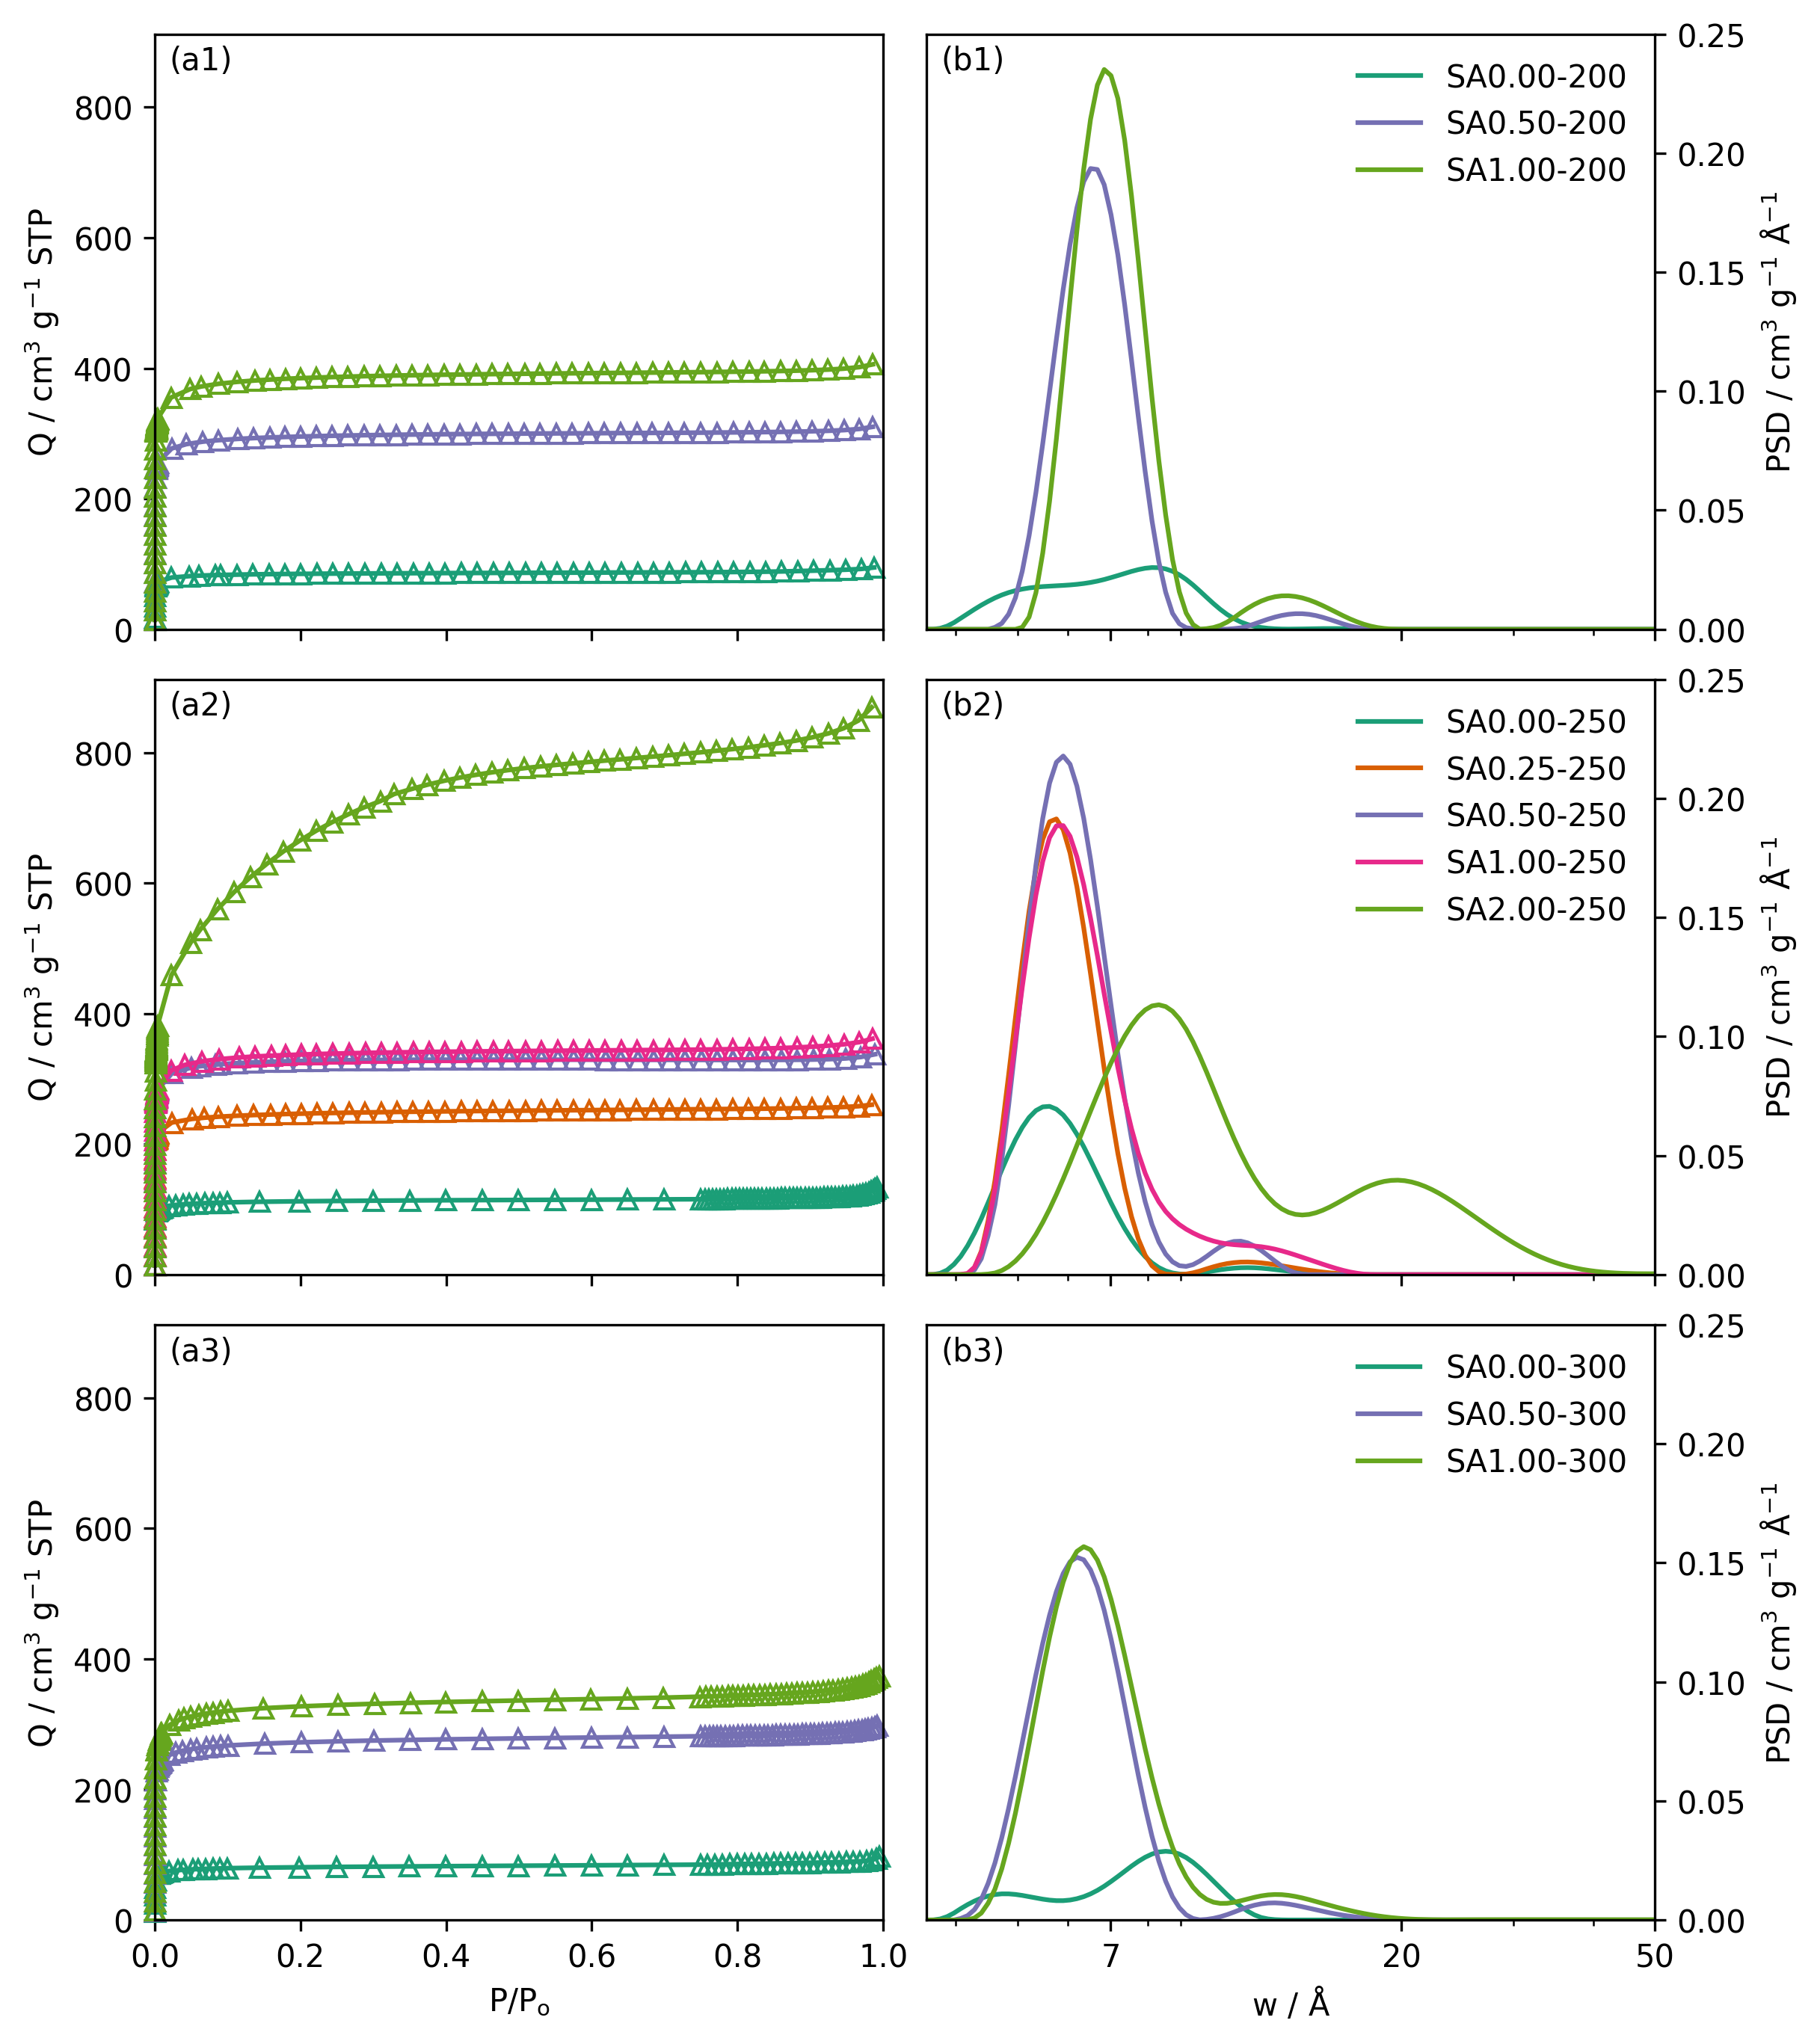
\includegraphics[width=\columnwidth, keepaspectratio]{4-impregnation/figs/SA_n2_isotherms.png}
    \caption{Isotherms (column a) and resultant \acrshortpl{psd} (column b) for SA samples hydrothermally carbonised at \qtylist[list-units=single]{200;250;300}{\degreeCelsius} (rows 1, 2 and 3 respectively).}
    \label{fig:SA_n2_isotherms}
\end{figure}

In the case of SA0.00-\textit{HHH} samples, overall surface area and pore volume (\qty{456}{\metre\squared\per\gram} and \qty{0.18}{\cm\cubed\per\gram}) was maximised where the \gls{htc} temperature was \qty{250}{\degreeCelsius}. Increasing \gls{htc} temperature generally reduces \ce{C} content in the resultant \gls{hydrochar},\citep{Sevilla2009a, parshetti2013chemical, kim2014hydrothermal} however temperatures above \qty{250}{\degreeCelsius} have also been shown to result in the break down of the poylmerised product into volatile organic moieties.\citep{gao2012characterization, Xiao2012Hydrothermal, wang2018review} As such, the apparent optimisation of porosity found by preparation with \gls{htc} at \qty{250}{\degreeCelsius} is likely a result of both of these factors affecting the activation resistance\citep{Altwala2020Predictable, Blankenship2022Modulating} and thus ultimately the porosity of the resultant activated carbon.

As for the \ce{KOH}-activated samples, in general increasing \ce{KOH}:\acrshort{sd} ratio is associated with increases in overall porosity, with SA2.00-250 achieving the highest surface area and pore volume of \qty{2396}{\metre\squared\per\gram} and \qty{0.84}{\cm\cubed\per\gram} respectively. In general this improvement does not appear to significantly affect microporosity which remains in the range \numrange[range-phrase={-}]{88}{94} and \qtyrange[range-units=single, range-phrase={-}]{81}{92}{\percent} in terms of surface area and pore volume respectively. This is, until \ce{KOH}:\acrshort{sd} ratio is increased to \num{2.00}, wherein development of mesoporosity reduces percent micropore surface area to \qty{27}{\percent}. This is reflected in the \ce{N2} isotherm for this sample (see figure \ref{fig:SA_n2_isotherms}(a2)) which displays a large \gls{adsorption} knee, unlike the very pure type I isotherms\citep{Thommes2015Physisorption} of the remaining samples.

The additional KOH:\acrshort{sd} ratio of 0.25 and 2.00 were included at \gls{htc} temperature of \qty{250}{\degreeCelsius} due to the relative similarity of isotherms and resultant porosities where KOH:\acrshort{sd} ratio is 0.50 or 1.00. In all cases, percent microporosity remains approximately the same, and the pore size is identical at these two ratios (see table \ref{tb:sa_porosity}). There are of course small improvements in overall porosity (most pronounced according to pore volume), when the ratio is increased from 0.50 to 1.00, but not to the extent that might be expected for a doubling of the amount of \gls{porogen} in the reaction mixture. This is most evident when examining differential \glspl{psd} (see figure \ref{fig:SA_n2_isotherms}(b1-3)) where for all SA\textit{x.xx-HHH} samples with \textit{x.xx} between 0.25 and 1.00 the profile is essentially the same, with porosity centered at \qtyrange[range-units=single, range-phrase={-}]{6}{8}{\angstrom}, and having minor shifts in position and/or size of the maximum which may simply be attributable to fitting of the kernel to the at times poorly equilibrated isotherm (see appendix, figures \ref{fig:SAxxx-200_isopsd}-\ref{fig:SAxxx-300_isopsd}). Similarly, for samples wherein \textit{x.xx} is 0.00, the \gls{psd} is much broader with low porosity at any given value of $w$, but all porosity remains in the \gls{micropore} region. Conversely, SA2.00-250 displays a clear hierarchical \gls{psd} with significant porosity in both the \gls{micropore} and small \gls{mesopore} range. 


In their 2017 work Balahmar \textit{et al.} report carbons which were synthesised by activation with \ce{KOH} at \qty{800}{\degreeCelsius} either of untreated sawdust or sawdust-derived \gls{hydrochar} synthesised at \qty{250}{\degreeCelsius}.\citep{Balahmar2017Biomass} Figure \ref{fig:SA_porosity_compare} compares these results. $A_{BET}$ is compared in terms of both \ce{KOH}:precursor mass ratio, and atomic \ce{K}:\ce{C} ratio; the latter according to the elemental composition of the precursor (sawdust or \gls{hydrochar}). The three methods, i.e. direct activation of sawdust, activation of \gls{hydrochar}, and hydrothermal impregnation of \ce{KOH} into sawdust do not seem to show any significant difference in terms of the overall $A_{BET}$ of the final product. Indeed, there is a clear strong linear correlation  between amount of \ce{KOH} used and $A_{BET}$; $r^2=0.90$, regardless of whether mass of \ce{KOH} or amount of \ce{K} is considered. The slopes of the linear regressions on figure \ref{fig:SA_porosity_compare}(a1, a2) are \qtylist[list-units=single]{523;386}{\metre\squared\per\gram}, respectively. Thus, increases in $A_{BET}$ with increasing amount of \ce{KOH} can be precisely predicted. Furthermore, the temperature used in the hydrothermal impregnation step (this work) does not significantly effect $A_{BET}$ of the final product. However, the microporosity of the product is significantly effected by synthetic method. At a \ce{KOH}:precursor mass ratio of 2.00, microporosity is maximised by direct activation of sawdust at \qty{84}{\percent}, which decreases to \qty{63}{\percent} for activation of sawdust-derived \gls{hydrochar}, and finally to \qty{27}{\percent} for the hydrothermal impregnation method. These results are also reflected by the very broad, principally mesoporous \gls{psd} of SA2.00-250 relative to the comparable samples reported in the paper by Balahmar and co-workers.\citep{Balahmar2017Biomass} 

\begin{landscape}
%\newpage
%\begin{rotate}{90}
\begin{SCfigure}%[hptb]
    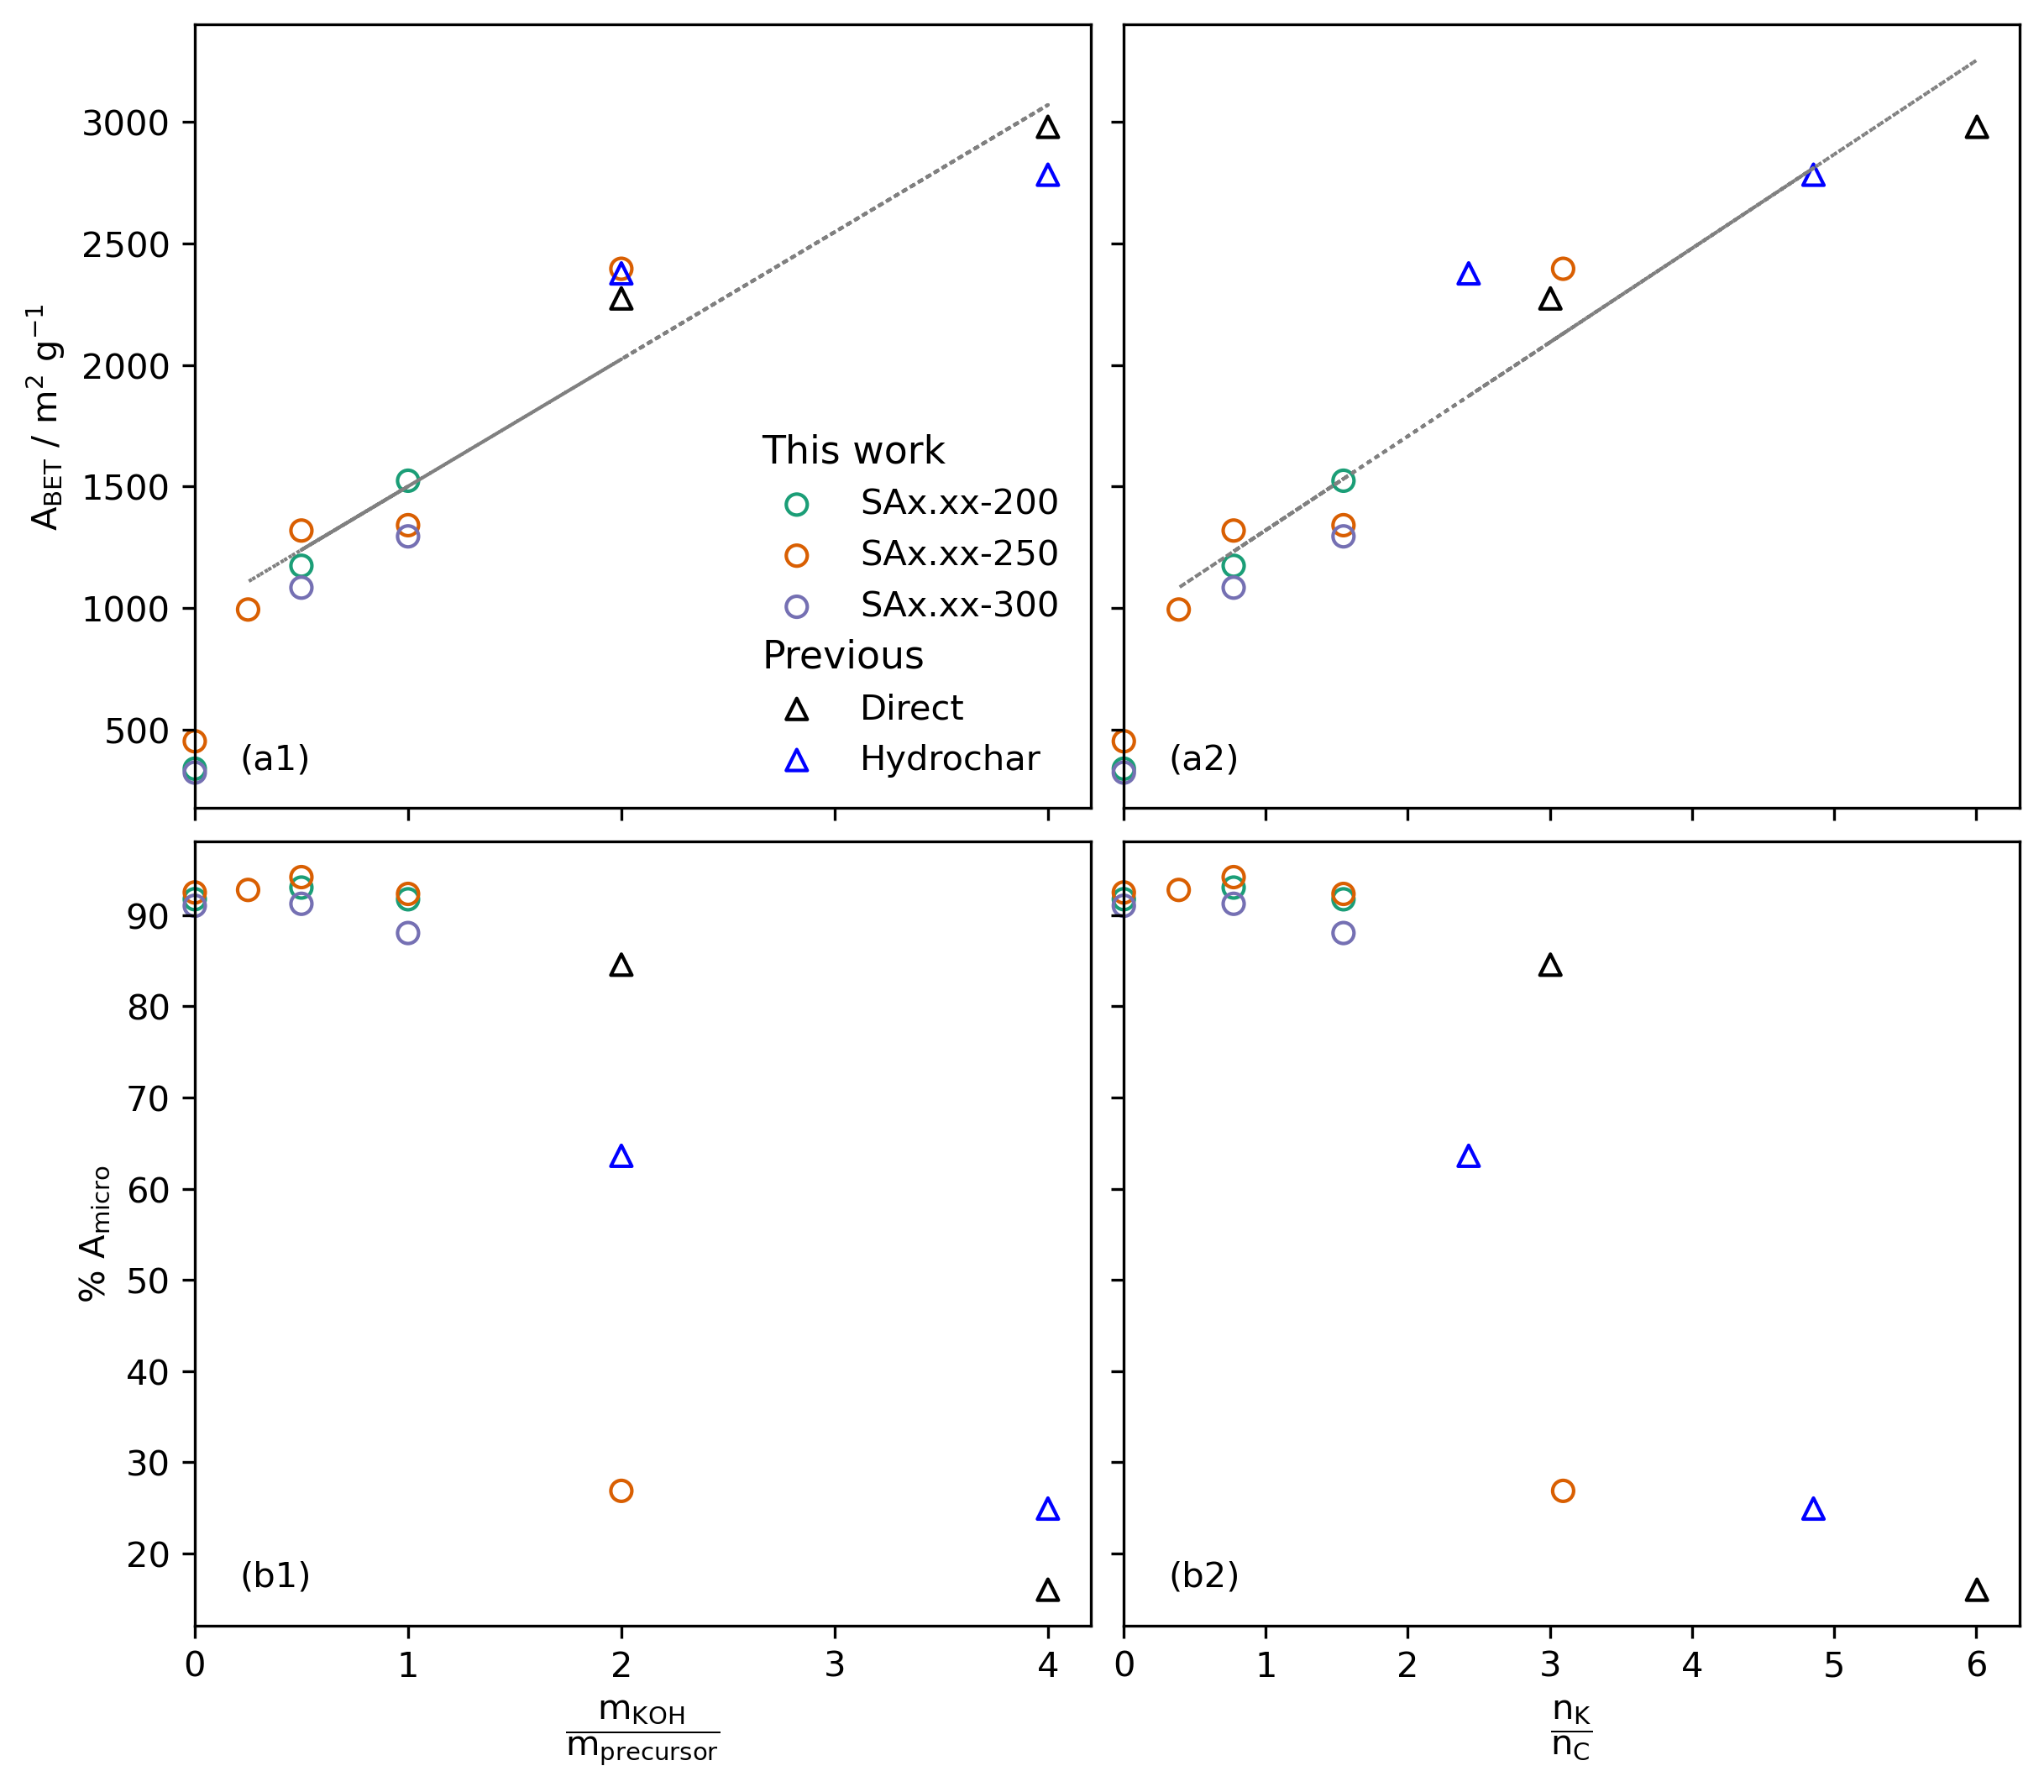
\includegraphics[width=0.55\paperheight, keepaspectratio]{4-impregnation/figs/SD_porosity_compare.png}
    \caption{\protect\rule{0ex}{5ex} Relationship between amount of \ce{KOH} used in activation of sawdust and porosity. Samples synthesised by Balahmar \textit{et al.} included to show effect of different methods of preparation.\citep{Balahmar2017Biomass} Amount of \ce{KOH} shown as KOH:precursor mass ratio (column 1), and as \ce{K}:\ce{C} atomic ratio (column 2). Porosity shown in terms of total $A_{BET}$ (row a) and micropore surface area calculated using t-plot (row b).}
    \label{fig:SA_porosity_compare}
\end{SCfigure}
%\end{rotate}
%\clearpage

\end{landscape}

\paragraph{Density}

\begin{figure}[b!]
    \centering
    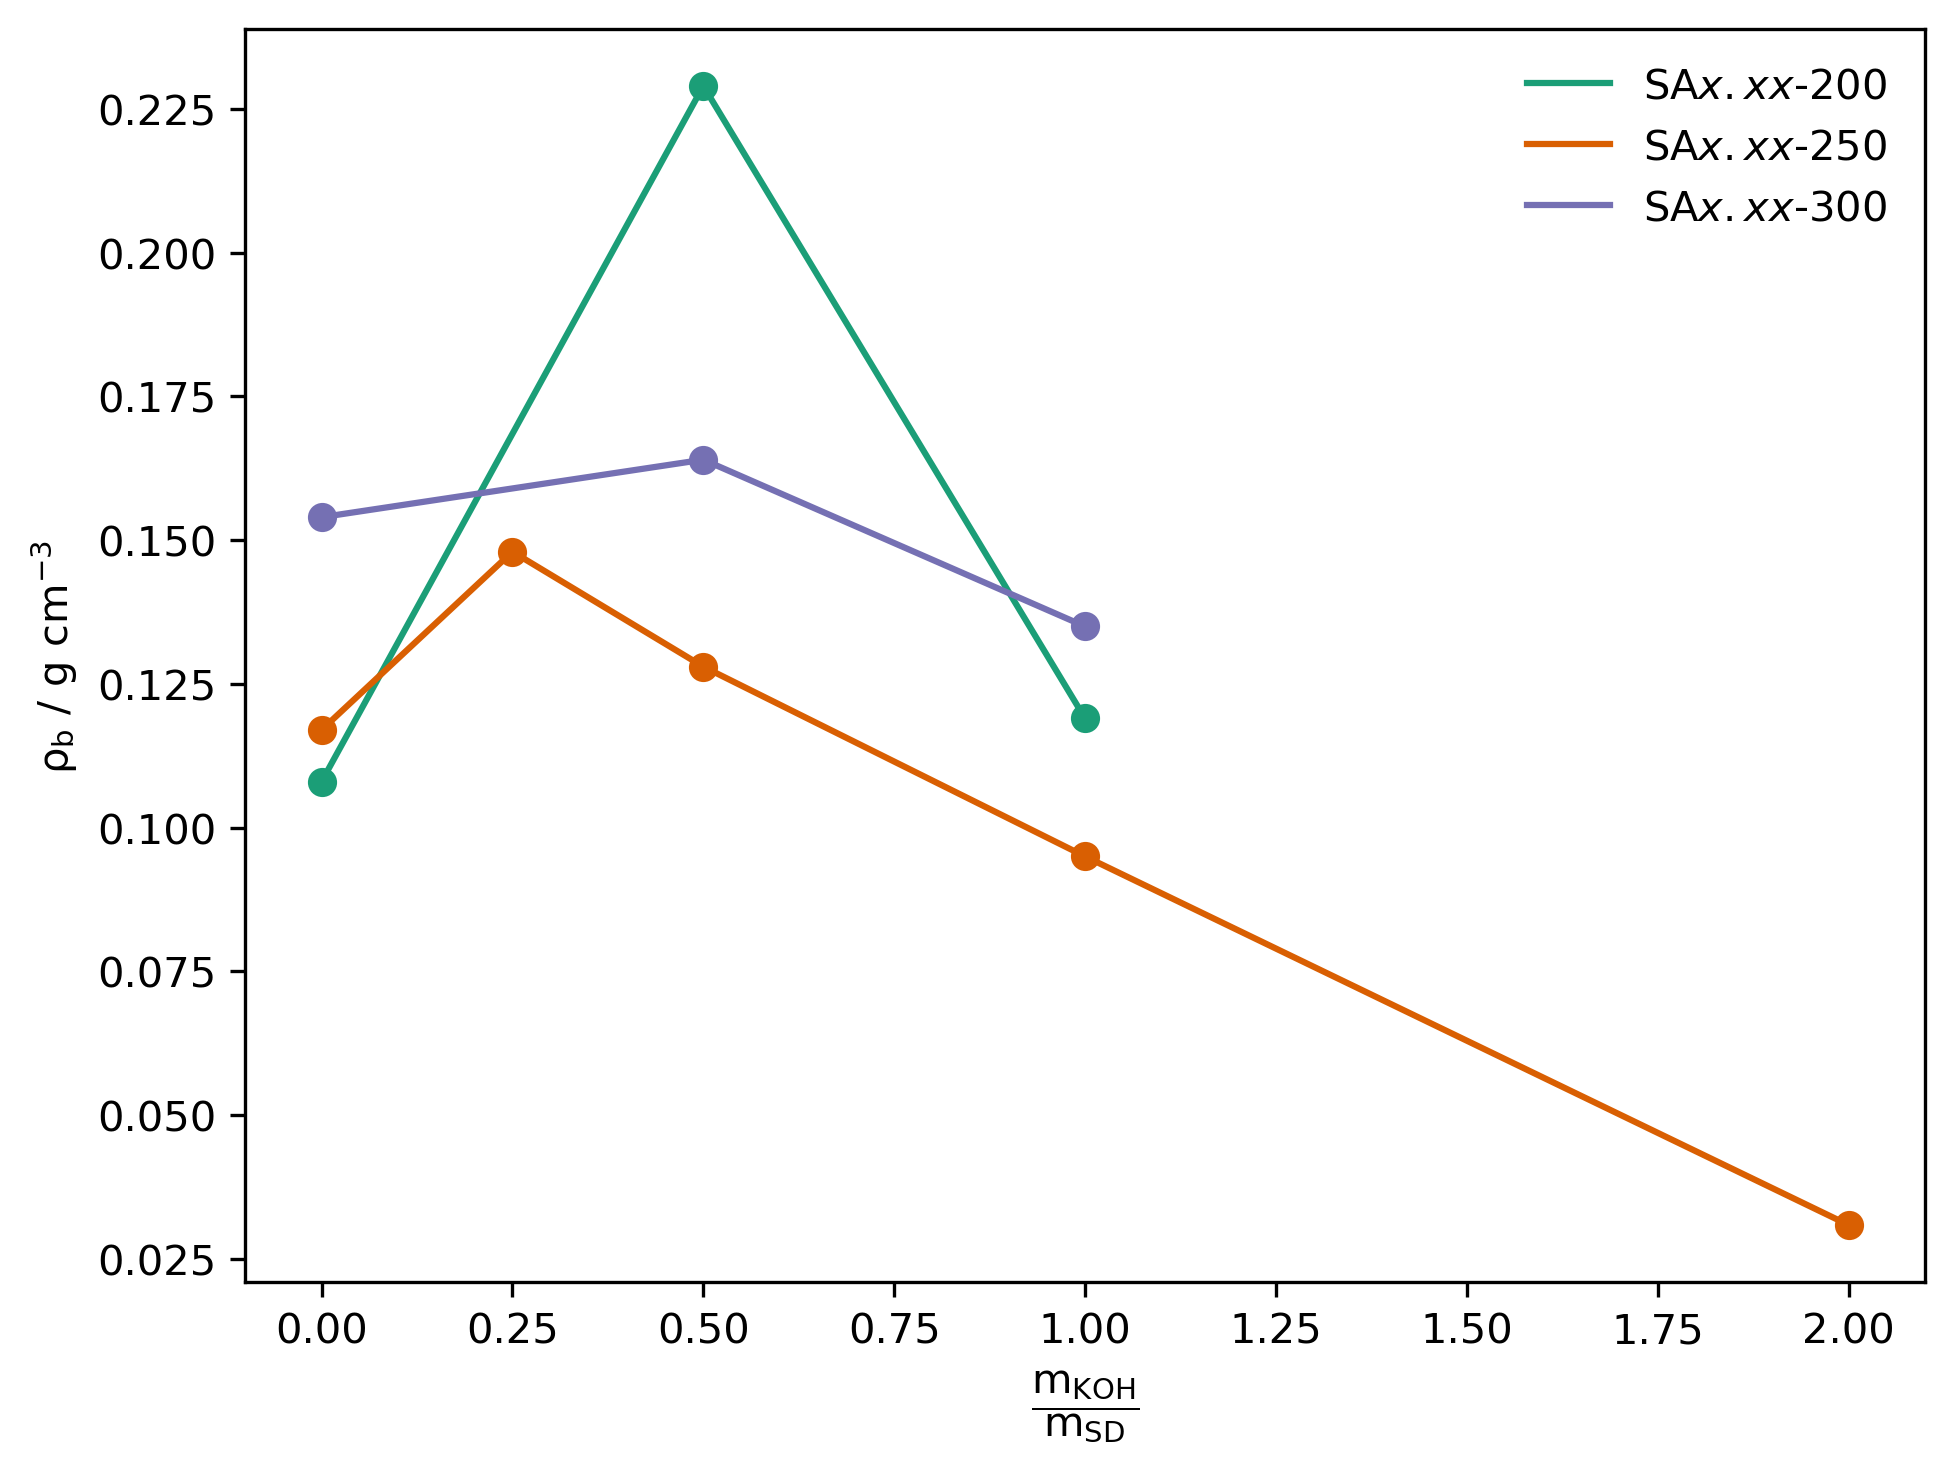
\includegraphics[width=\columnwidth, keepaspectratio]{4-impregnation/figs/SD_density.png}
    \caption{Effect of \ce{KOH}:\acrshort{sd} ratio on bulk density, $\rho_b$ of carbons synthesised using the three \ce{htc} temperatures. $\rho_b$ estimated from freespace measurements.}
    \label{fig:SA_density}
\end{figure}

As mentioned in section \ref{ss:sd_results}, sample SA2.00-250 was noticeably more diffuse than the other samples. In lieu of access to appropriate pycnometric equipment, bulk density ($\rho_{b}$) of samples found here was estimated by using ambient temperature \ce{He} freespace measurements used to calibrate the measurement of \ce{N2} isotherms. The sample volume was taken as the difference between this freespace and the ambient freespace of the empty tube, thus calculation of the $\rho_{b}$ was trivial as sample mass is already known. These estimated bulk densities are shown in figure \ref{fig:SA_density}. Densities of these carbons are at the low end of that  reported for \ce{KOH}-activated carbons,\citep{casco2015very, machnikowski2012adsorption, Altwala2020Predictable} however similar values have been reported by some groups.\citep{tseng2008effects, rashid2016koh, Guan2011Methane} Additionally, for \ce{KOH} activated samples, $\rho_b$ is negatively correlated with amount of \ce{KOH} used during activation, similarly to reports by Tseng \textit{et al.}.\citep{tseng2008effects} The extremely low bulk density (\qty{0.031}{\gram\per\cm\cubed}) of SA2.00-250 may be ascribed to an effect described by Deng and co-workers in 2015, i.e. that high production of gases by the activating agent results in bulk densities as low as \qty{0.043}{\gram\per\cm\cubed} and hierarchical \glspl{psd}.\citep{Deng2015Inspired} While the gas production in the work by Deng \textit{et al.} is thought to be a result of decomposition of the \ce{KHCO3} \gls{porogen}, in this study reactions of excess aqueous \ce{KOH} with the precursor during the hydrothermal impregnation step may form \glspl{porogen} that have a similar capacity to release gases such as \ce{CO2}. This does not however serve to explain the low densities of the remaining samples which are almost exclusively microporous. 

\newpage
\section{Sodium Carboxymethyl Cellulose}
\label{ss:NC}

Twelve carbon samples were produced from sodium carboxymethyl cellulose with varying \acrshort{ds}. On removal from the furnace, samples derived from precursors containing \ce{Na} glowed red due to exposure of small amounts of elemental \ce{Na} to air, thus indicating this species is a product of the activation process. While there is some debate as to whether elemental metals form during activation with \ce{KOH} or \ce{NaOH},\citep{Blankenship2022Modulating, Sevilla2014Energy, LozanoCastello2007Carbon, Kelemen1983interaction, Xue2003Formation} it is clear that it occurs here. In addition, these samples took the form of a single, hard mass whereas activated carbons are typically powders. On washing with \ce{HCl}, the samples broke up into a fine powder. This indicates that residual \ce{Na} compounds or other by-products of activation may be holding particles together in some way.

\subsection{Composition}
\label{sss:NC_composition}

\begin{figure}[htpb!]
    \centering
    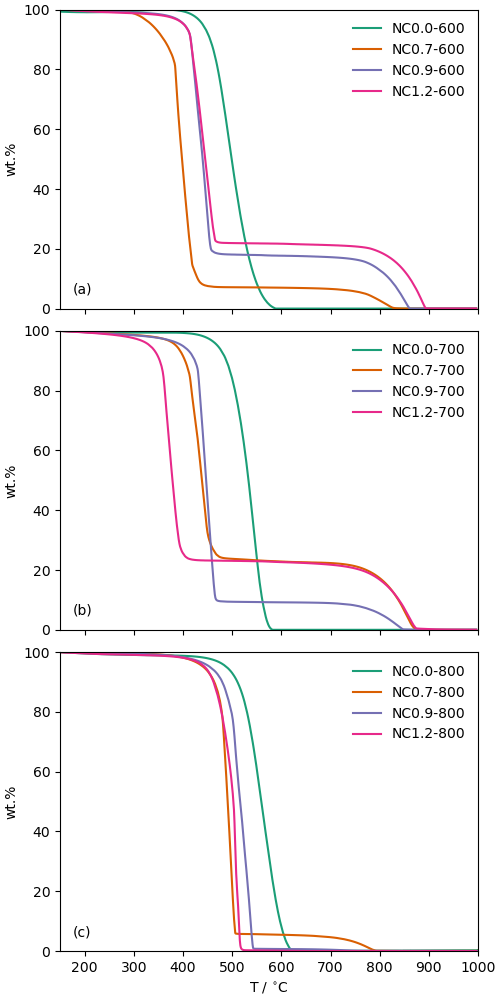
\includegraphics[width=0.82\columnwidth, keepaspectratio]{4-impregnation/figs/NC_tga_adj.png}
    \caption{\acrshort{tga} curves for all NC\textit{x.x-TTT} samples, adjusted for water evaporation, and residual masses set to 0, where within \qty{1}{\wtpercent}. Original (unadjusted) thermograms are provided in figure \ref{fig:NC_tga}.}
    \label{fig:NC_tga_adj}
\end{figure}

\acrshort{tga} (shown in figure \ref{fig:NC_tga_adj}) of the twelve samples confirms that the washing process removed any residual \ce{Na} compounds, i.e. the samples are all fully carbonaceous. In order to simplify direct comparisons between the combustion behaviour of the samples, the initial mass loss (moisture loss) at \qty{100}{\degreeCelsius} is ignored, and initial mass is taken to be that of the dry sample. In addition, the residual mass has been adjusted to \qty{0}{\wtpercent} for all samples to improve plot readability.\footnote{Unadjusted \acrshort{tga} curves can be found in the appendix, figure \ref{fig:NC_tga}.} For some of the \glspl{turbostratic carbon} there is a large loss of mass at between \qtylist[list-units=single]{400;500}{\degreeCelsius}, before the remainder of the sample is burned off. This is followed by a second burn-off event between \qtylist[list-units=single]{800;900}{\degreeCelsius}. In the case of samples with only a single burn-off temperature, this occurs at between \qtylist[list-units=single]{500;650}{\degreeCelsius}. The dual burn-offs appear to be associated with the presence of \ce{Na} in the precursor, as all NC0.0-\textit{TTT} samples only display a single-burn off. Furthermore, both the amount of \ce{Na} in the precursor and the activation temperature influence the temperature and mass decrease in the first mass loss (when it is present). For example, for NC\textit{x.x}-600 samples, the mass loss associated with the initial burn-off decreases with increasing \acrshort{ds}, while the temperature of this process increases. The trend for NC\textit{x.x}-700 is more convoluted, and for NC\textit{x.x}-800 samples only NC0.7-800 displays the dual burn-off behaviour. Nonetheless, it appears that the oxidative \gls{porogen} (here in the form of \ce{Na} and/or \ce{CH2COONa} and/or other various derivatives) produces two phases in the resultant carbons to varying extents depending on the activation temperature and \ce{Na}:\ce{C} ratio. 

\begin{figure}[hptb]
    \centering
    \captionof{table}{Composition of sodium carboxymethyl cellulose at all values of \acrshort{ds}, and of NC\textit{x.x-TTT} carbons according to CHN elemental microanalysis. For NC\textit{x.x-TTT} carbons, \ce{O} content is taken as remainder of the sum of \ce{C} and \ce{H} contents as samples are clean according to \acrshort{tga}. \ce{N} content not shown as it is zero for all samples.}
    \label{tb:nc_chn}
    \begin{tabularx}{0.9\textwidth}{lXXXXXXX}
    \toprule
        \textbf{Sample} & \multicolumn{4}{c}{\textbf{Concentration / \unit[detect-weight]{\wtpercent}}} & \multicolumn{3}{c}{\textbf{Atomic ratio}} \\
        & \textbf{C} & \textbf{H} & \textbf{O} & \textbf{Na} & \textbf{O/C} & \textbf{H/C} & \textbf{Na/C} \\
    \midrule
        \textbf{NC0.0} & 44 & 6.2 & 49 & 0 & 0.83 & 0.14 & - \\
        \textbf{NC0.0-600} & 87 & 1.9 & 11 & 0 & 0.10 & 0.26 & - \\
        \textbf{NC0.0-700} & 91 & 0.97 & 8.5 & 0 & 0.07 & 0.13 & - \\
        \textbf{NC0.0-800} & 92 & 0.46 & 7.4 & 0 & 0.06 & 0.06 & - \\
        \\
        \textbf{NC0.7} & 41 & 5.2 & 47 & 7.4 & 0.87 & 0.13 & 0.09 \\
        \textbf{NC0.7-600} & 76 & 2.8 & 21 & 0 & 0.21 & 0.43 & - \\
        \textbf{NC0.7-700} & 65 & 0.38 & 35 & 0 & 0.40 & 0.07 & - \\
        \textbf{NC0.7-800} & 85 & 0.37 & 15 & 0 & 0.13 & 0.05 & - \\
        \\
        \textbf{NC0.9} & 40 & 5.1 & 46 & 8.8 & 0.88 & 0.13 & 0.12 \\
        \textbf{NC0.9-600} & 83 & 0.26 & 17 & 0 & 0.16 & 0.04 & - \\
        \textbf{NC0.9-700} & 75 & 0.36 & 25 & 0 & 0.25 & 0.06 & - \\
        \textbf{NC0.9-800} & 90 & 0.3 & 9.5 & 0 & 0.08 & 0.03 & - \\
        \\
        \textbf{NC1.2} & 39 & 4.8 & 46 & 11 & 0.89 & 0.12 & 0.14 \\
        \textbf{NC1.2-600} & 66 & 0.89 & 33 & 0 & 0.38 & 0.16 & - \\
        \textbf{NC1.2-700} & 64 & 0.61 & 36 & 0 & 0.42 & 0.11 & - \\
        \textbf{NC1.2-800} & 76 & 0.06 & 24 & 0 & 0.24 & 0.01 & - \\
    \bottomrule
    \\
    \end{tabularx}

    \centering
    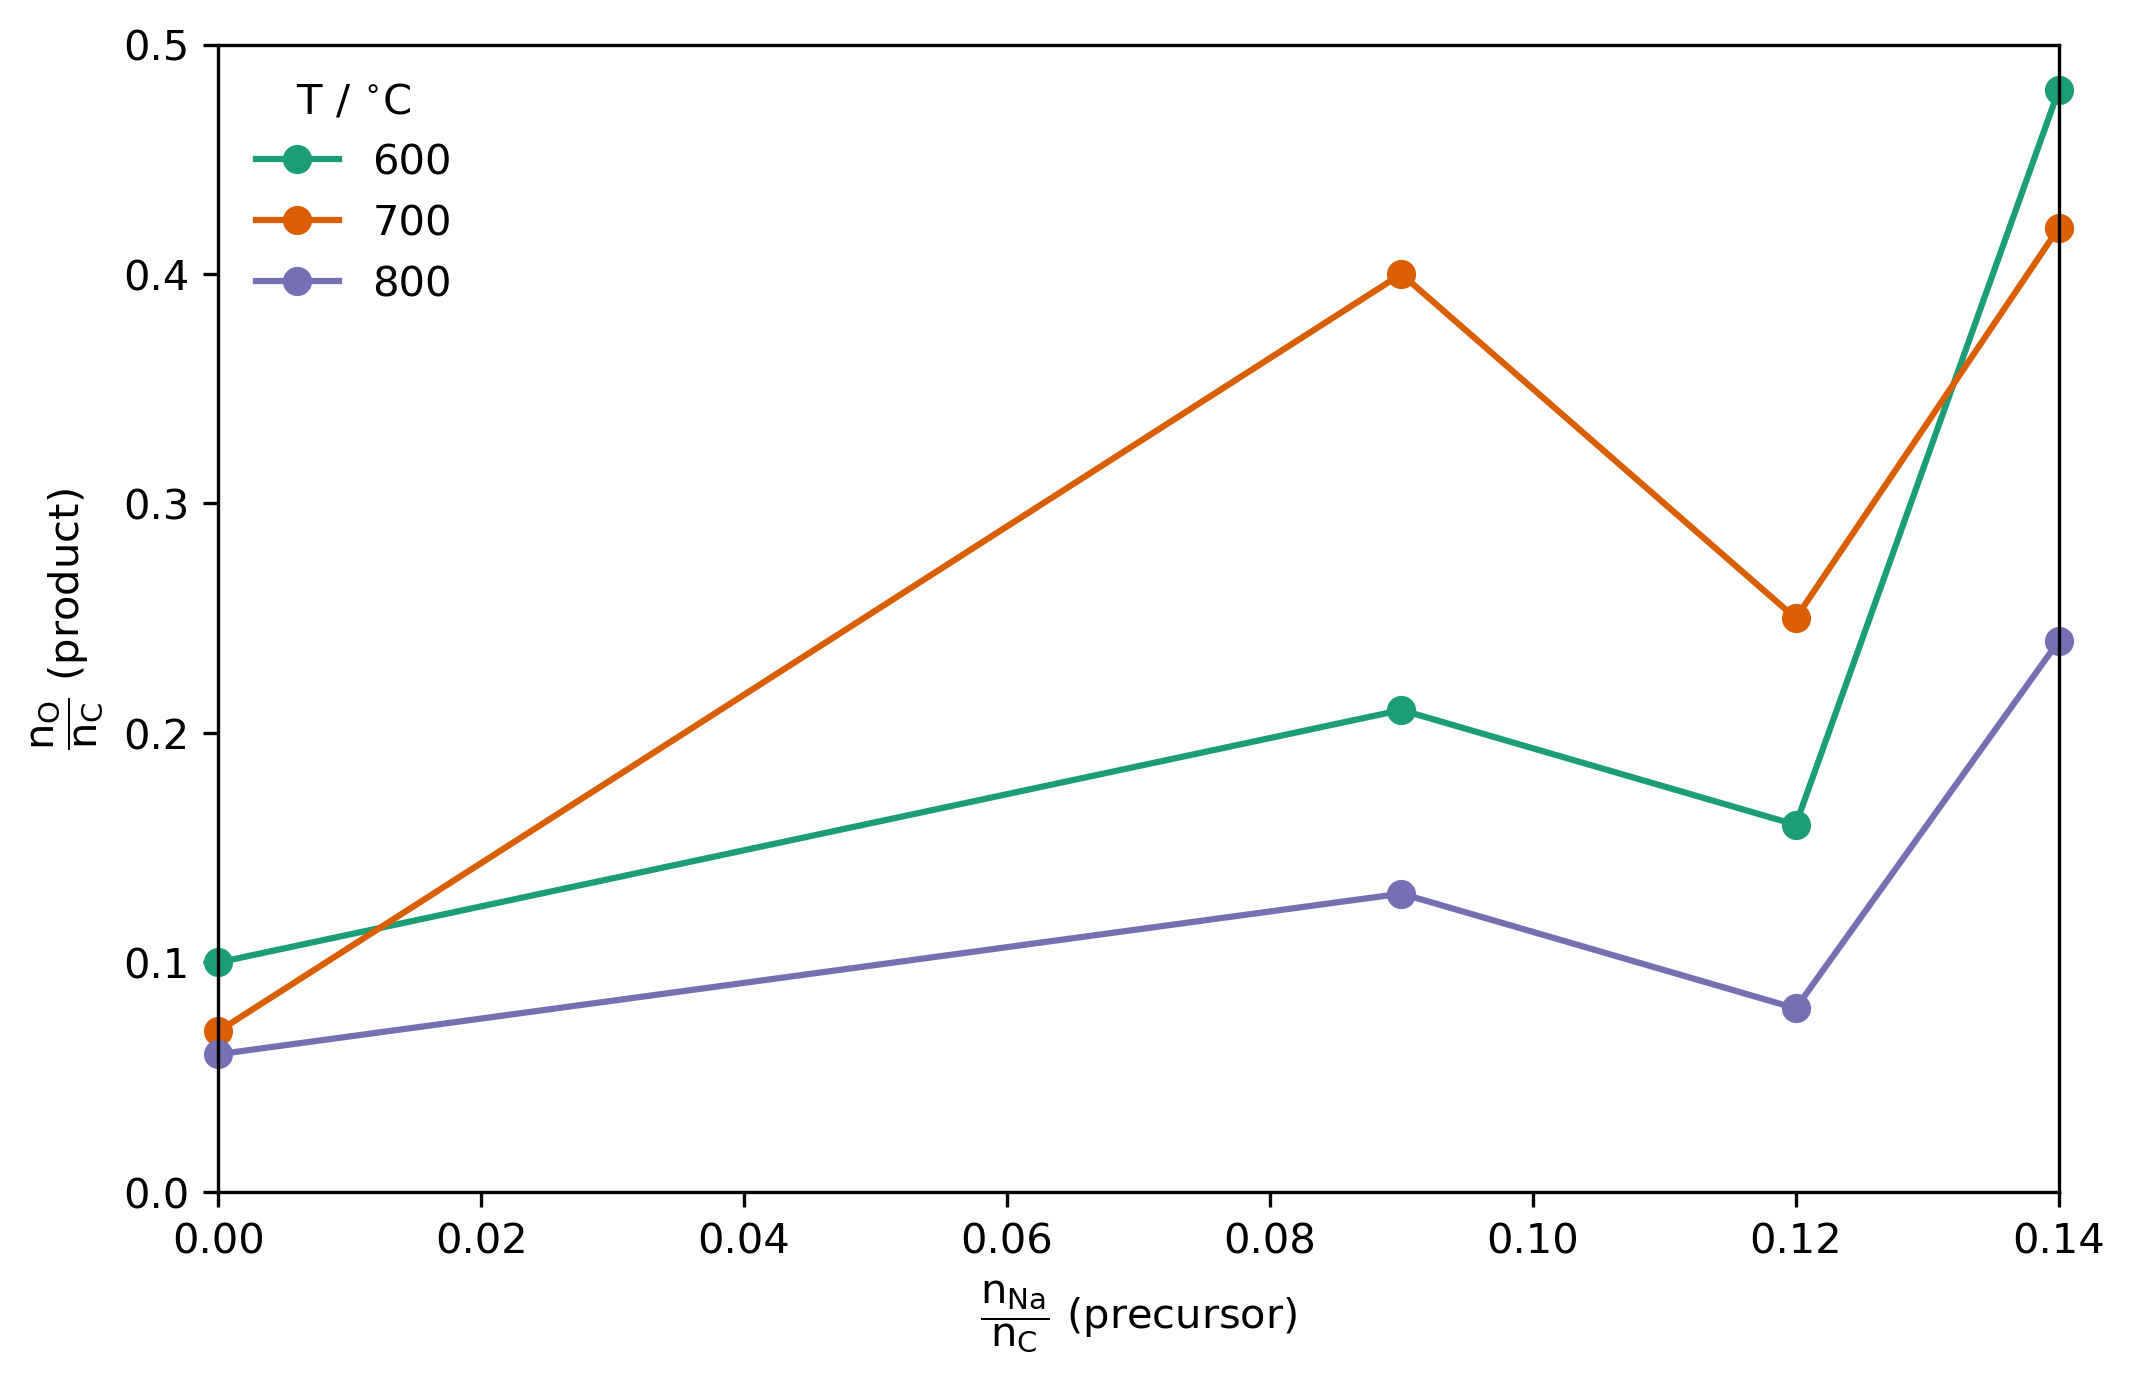
\includegraphics[width=\columnwidth, keepaspectratio]{4-impregnation/figs/NaCprecursor_OCproduct.png}
    \captionof{figure}{The effect of precursor \ce{Na}:\ce{C} ratio on the \ce{O}:\ce{C} ratio in the product at each of the three pyrolysis temperatures, $T$.}
    \label{fig:NaCprecursor_OCproduct}
\end{figure}

Results of CHN elemental microanalysis are shown in table \ref{tb:nc_chn}, alongside calculated concentrations of \ce{C}, \ce{H}, \ce{O}, and \ce{Na} in each of the four precursors. While there are variations in \ce{C}, \ce{H} and \ce{O} content between the four precursors, the most significant change is with respect to the \ce{Na}:\ce{C} ratio. The effect of precursor \ce{Na}:\ce{C} ratio on product \ce{O}:\ce{C} ratio is shown in figure \ref{fig:NaCprecursor_OCproduct}. Typically, increased oxidative \gls{porogen} concentration results in higher relative \ce{O} contents in the derived porous carbon, commonly believed to be due to increased destruction of the \ce{C} framework.\citep{park2002effect, chen2020insight, tseng2007physical} What is interesting in the case of these sodium carboxymethyl cellulose-derived carbons is that there is a consistent minimum in atomic \ce{O}:\ce{C} ratio for carbons derived from precursors with a \ce{Na}:\ce{C} of 0.12, i.e. a \acrshort{ds} of 0.9, regardless of activation temperature. The effect of quantity of \gls{porogen} on the mechanism of oxidative chemical activation is not typically investigated for such low \gls{porogen}:\ce{C} ratios, so there is little to base a mechanistic hypothesis on for this case. However, it is possible that there is a balance being struck between formation of cross-links and activation with the \ce{Na+} cation (or its derivatives). Cross-link formation, if it occurs ought to result in the loss of \ce{O} due to the condensation of the two carboxylate groups to form the anyhdride linkage. Thus the drop in the \ce{O} concentration at a \acrshort{ds} of 0.9 may indicate the dominance of the (\ce{O}-removing) cross-linking process over the (\ce{O}-increasing) oxidative action of the \gls{porogen}. Similarly, the high \ce{O} content of samples synthesised at \qty{700}{\degreeCelsius} relative to the other two temperatures may be a function of the two competitive mechanisms. That is, pyrolysis at \qty{700}{\degreeCelsius} is optimal for cross-link formation. It should be noted however, that cross-linkages between sodium carboxymethyl cellulose chains have thus far only been shown to form as a result of low temperature, solution phase reactions with the use of reagents to promote their formation.\citep{lin2015preparation, yu2017koh, yu2017one}

\subsection{Porosity}

The samples in this work were not expected to have a high degree of porosity, and thus not expected to be particularly suitable candidates for gas sorption applications. Classical measures of porosity of the twelve carbons are displayed in table \ref{tb:nc_porosity}, and the \ce{N2} isotherms from which these quantities are derived as well as the resultant \acrshort{psd}s are shown in figure \ref{fig:NC_n2_isotherms}. Full details of \acrshort{psd}s and fitting to \acrshort{nldft} kernels are shown in the appendix, figures \ref{fig:NCxx-600_psdisofull}-\ref{fig:NCxx-800_psdisofull}.\footnote{Due to poor equilibration, these \acrshortpl{psd} cannot be considered to be accurate, this is discussed in more depth in chapter \ref{ch:dual_isotherm} and \ref{pub:dual_iso}.} Most samples are highly microporous according to t-plot calculations, having 87-91 \% and 75-90 \% \gls{micropore} surface area and pore volume respectively. The notable exceptions to this are NC0.7-600 wherein $A_{BET}$ and $V_t$ are so low that t-plot calculations are rendered extremely imprecise, as well as NC1.2-600 and NC1.2-800. The slightly lower microporosity of the latter two samples may be attributed to increased \gls{mesopore} development due to higher quantities of \gls{porogen}. 

\begin{table}[ht!]
    \caption{Porosity of NC\textit{x.x-TTT} carbons. $A_{BET}$ derived using the Rouquerol method. The total pore volume, $V_t$ is taken using the single point method. Values in brackets indicate the microporous portion of $A_{BET}$ and $V_t$, calculated using t-plot. Peak pore width $w_{peak}$ is the maximum of the \acrshort{psd} determined using \acrshort{nldft}, as shown in figure \ref{fig:NC_n2_isotherms}.}
    \label{tb:nc_porosity}
    \begin{tabularx}{\textwidth}{Xllllll}
    \toprule
        \textbf{Sample} & \multicolumn{2}{l}{$\mathbf{A_{BET}}$ \textbf{/ \unit[detect-weight]{\metre\squared\per\gram}}}  & \multicolumn{2}{l}{$\mathbf{V_t}$ \textbf{/ \unit[detect-weight]{\cm\cubed\per\gram}}} & \multicolumn{2}{l}{$\mathbf{w_{peak}}$ \textbf{/ \unit{\angstrom}}} \\
    \midrule
        \textbf{NC0.0-600} & 587 & (530, 90\%) & 0.24 & (0.21, 88\%) & 6 \\
        \textbf{NC0.7-600} & 21 & (13, 62\%) & 0.01 & (-) & 7 \\
        \textbf{NC0.9-600} & 577 & (505, 88\%) & 0.25 & (0.19, 76\%) & 6 \\
        \textbf{NC1.2-600} & 238 & (213, 89\%) & 0.10 & (0.08, 80\%) & 6 \\
        \\
        \textbf{NC0.0-700} & 531 & (485, 91\%) & 0.21 & (0.19, 90\%) & 6 \\
        \textbf{NC0.7-700} & 162 & (151, 93\%) & 0.07 & (0.06, 85\%) & 7 \\
        \textbf{NC0.9-700} & 364 & (325, 89\%) & 0.16 & (0.13, 81\%) & 7 \\
        \textbf{NC1.2-700} & 190 & (169, 89\%) & 0.08 & (0.06, 75\%) & 5 \\
        \\
        \textbf{NC0.0-800} & 403 & (356, 88\%) & 0.17 & (0.13, 76\%) & 6 \\
        \textbf{NC0.7-800} & 491 & (427, 87\%) & 0.21 & (0.16, 76\%) & 6 \\
        \textbf{NC0.9-800} & 650 & (570, 87\%) & 0.28 & (0.22, 79\%) & 6 \\
        \textbf{NC1.2-800} & 476 & (382, 80\%) & 0.21 & (0.15, 71\%) & 5 \\
    \bottomrule
    \end{tabularx}
\end{table}

There are some clear trends with respect to overall porosity and both quantities of activating agent and activation temperature. The porosity of NC0.0-\textit{TTT} samples decreases with increasing activation temperature, while maintaining fairly constant microporosity (\qty{90(2)}{\percent}, by surface area), and average pore size of \qty{6}{\angstrom}. This indicates that for \glspl{biochar}, increasing activation temperature only serves to destroy porosity created at lower temperatures, while not broadening the \acrshort{psd} significantly. It has been previously observed that \gls{biochar} porosity is optimised with \gls{pyrolysis} temperature of around \qty{600}{\degreeCelsius},\citep{zama2017role, ronsse2013production, leng2021overview} although values for $A_{BET}$ and $V_t$ in these reports are around an order of magnitude less than shown by carbons reported herein from cellulose. Indeed, Zhang \textit{et al.} reported $A_{BET}$ and $V_t$ of only \qty{4.1}{\metre\squared\per\gram} and \qty{0.02}{\cm\cubed\per\gram} respectively for a carbon derived from the pyrolysis of cellulose at \qty{800}{\degreeCelsius},\citep{zhang2021pyrolysis} compared to the $A_{BET}$ of \qty{403}{\metre\squared\per\gram} for NC0.0-800. The samples reported here are more comparable in terms of porosity to that of the \gls{biochar} reported in chapter \ref{ch:cbs} derived from pure cellulose acetate (see table \ref{tb:CA_porosity}). This much higher surface area may simply be a result of washing of the biochars, which removes some soluble matter that contributed to pore blocking but may also be indicative of the low activation resistance of purely cellulosic materials relative to the traditionally carbonised ligno-cellulosic biomass.\citep{Hirst2018simple, Balahmar2019Pre, Zhang2019situ, Deng2016Effects} 

\begin{figure}[t!]
    \centering
    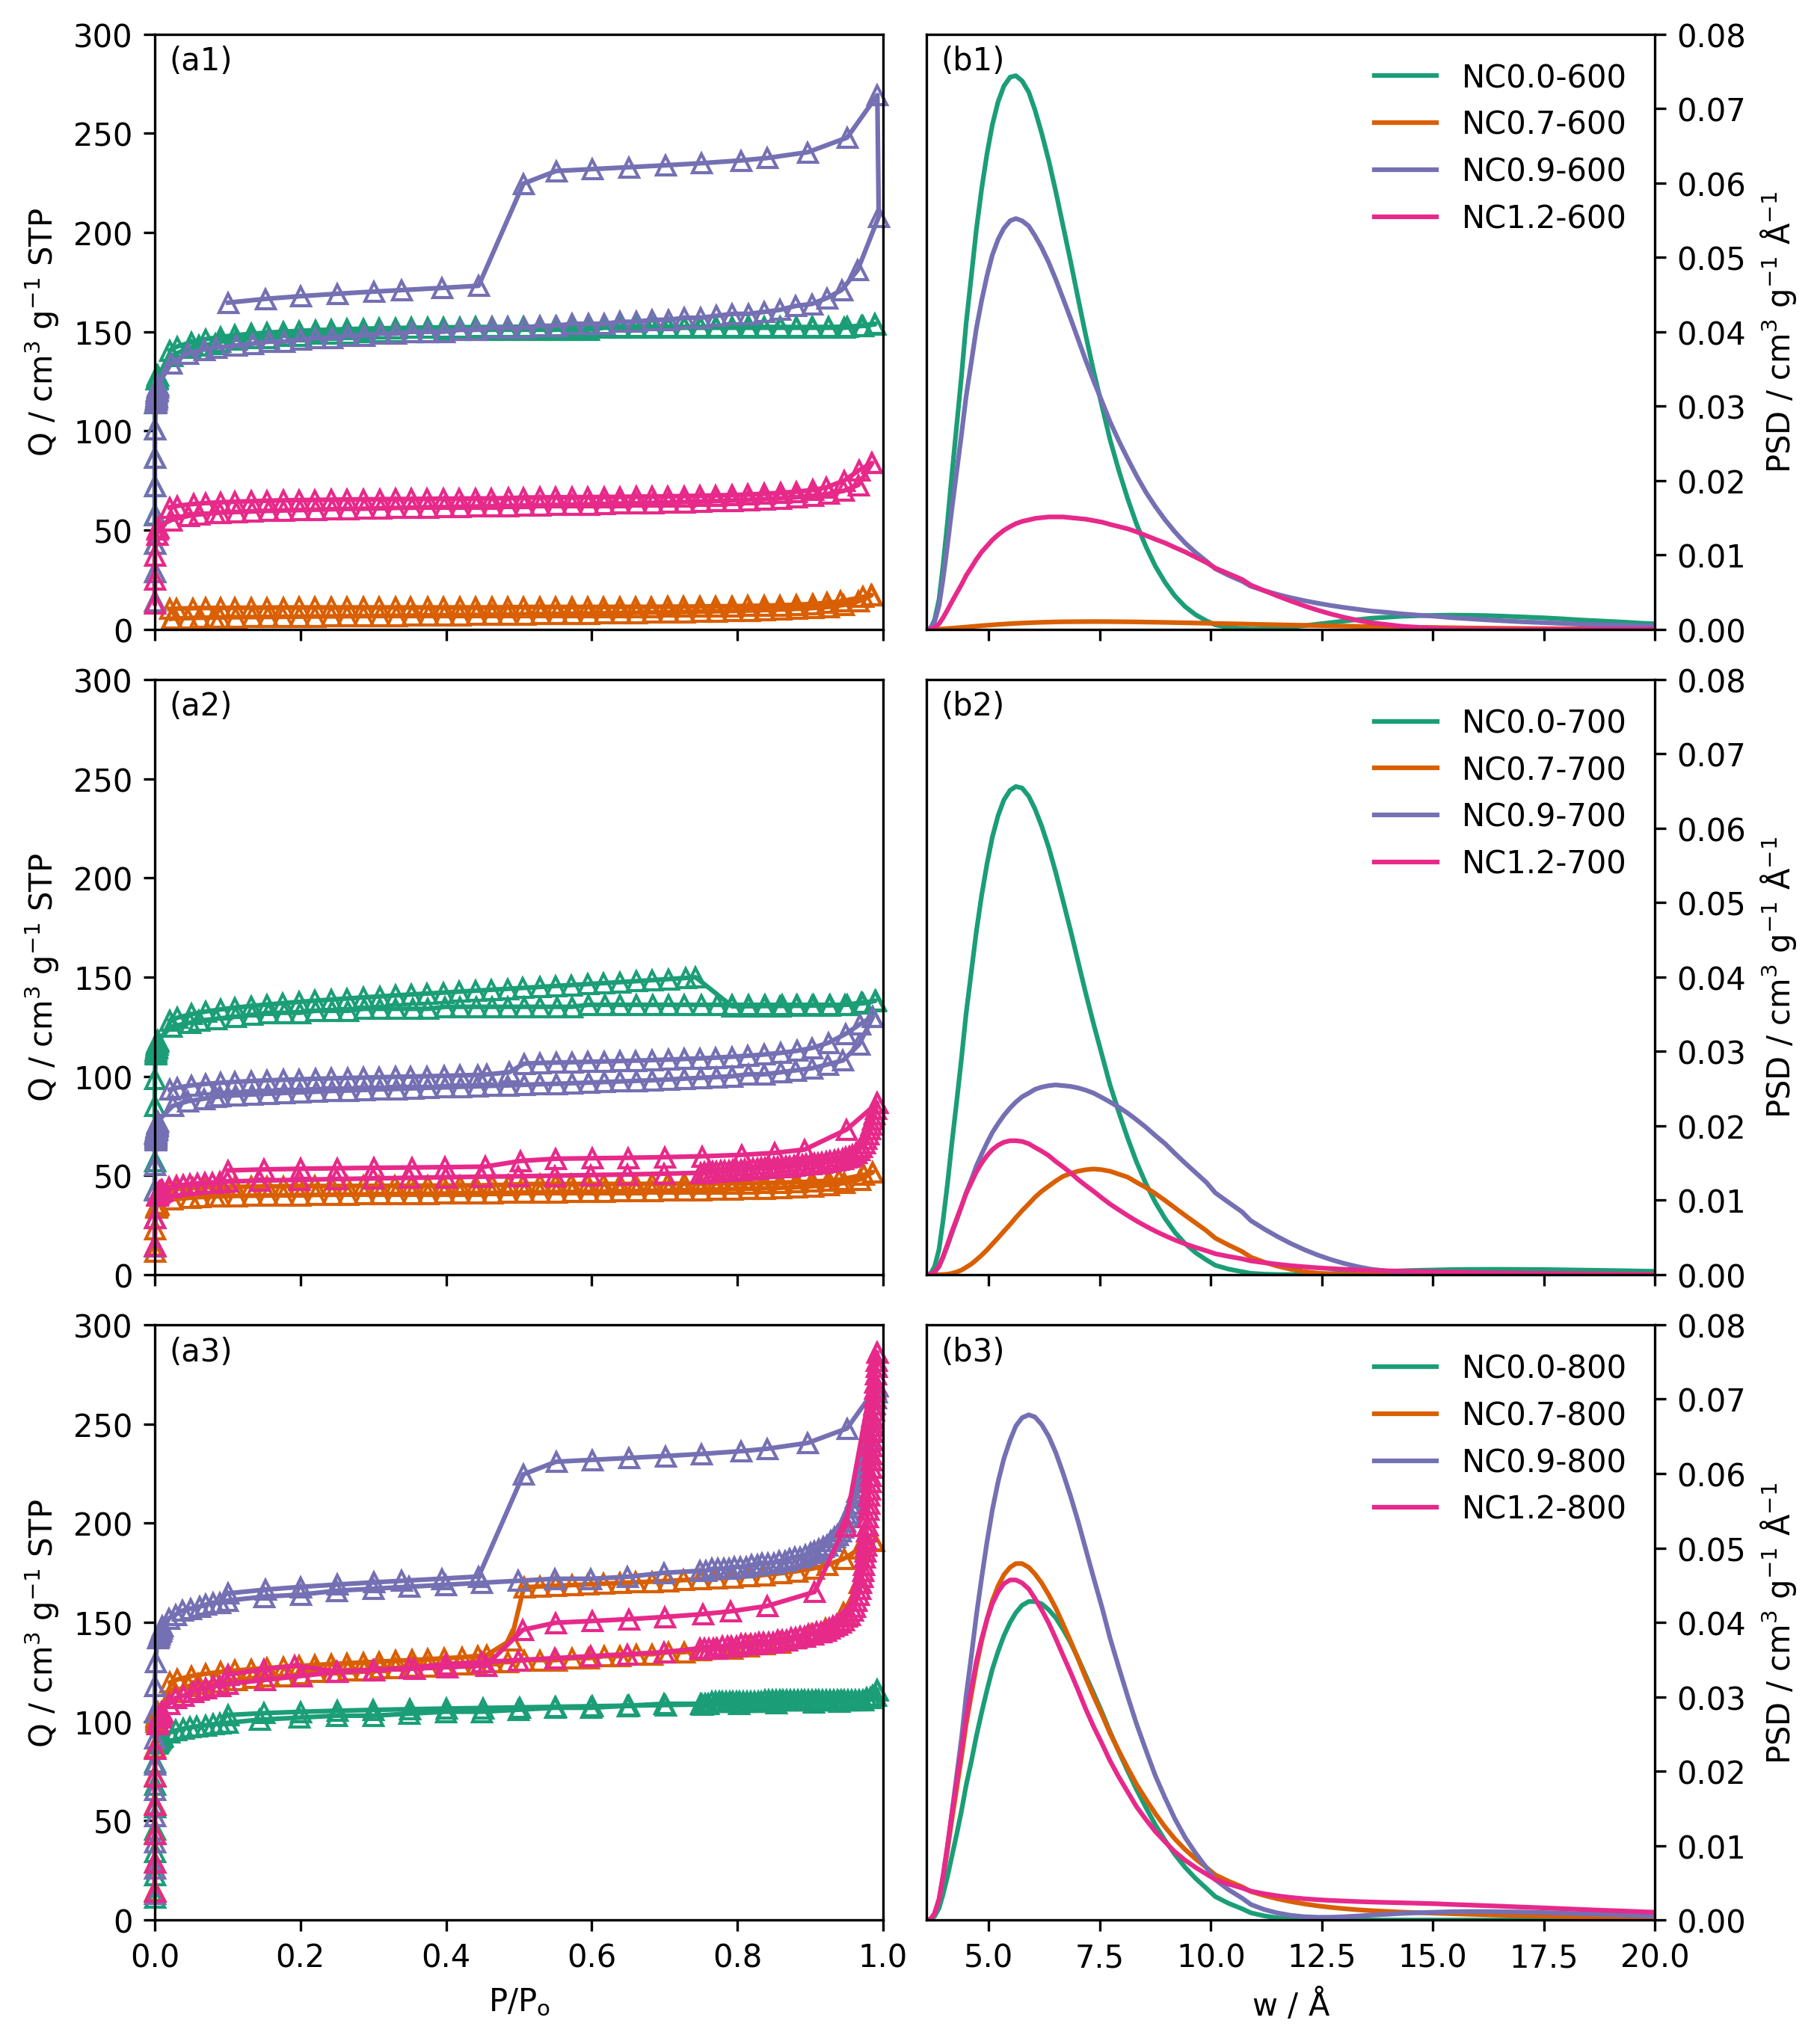
\includegraphics[width=\columnwidth, keepaspectratio]{4-impregnation/figs/NC_n2_isotherms.png}
    \caption{Isotherms (column a) and resultant PSDs (column b) for \acrshort{nc} samples activated at 600 (row 1), 700 (row 2), and 800 (row 3) \unit{\degreeCelsius}.}
    \label{fig:NC_n2_isotherms}
\end{figure}

Carbons derived from sodium carboxymethyl cellulose with a \acrshort{ds} between 0.7 and 1.2 consistently showed highest porosity at \acrshort{ds} of 0.9. While there is typically some optimum porogen:\ce{C} ratio for activation with \ce{NaOH} or \ce{KOH}, it is usually much higher than the extremely low value reported here.\citep{Sevilla2014Energy, Balahmar2017Biomass, tseng2006mesopore, Singh2019CO2, Boujibar2018CO2} A \acrshort{ds} of 0.9 corresponds to  an atomic \ce{Na}:\ce{C} ratio of just 0.12, while Balahmar \textit{et al.} reported that directly activated carbons from sawdust showed much higher $A_{BET}$ (\qty{1202}{\metre\squared\per\gram}) at a \ce{K}:\ce{C} atomic ratio of 0.19, which more than doubled when the amount of \gls{porogen} was doubled.\citep{Balahmar2017Biomass} Similarly, Tseng found that $A_{BET}$ of corn cob char-derived carbons was maximised at \qty{2500}{\metre\squared\per\gram} using a \ce{Na}:\ce{C} atomic ratio of 0.83. Indeed $V_t$ continued to increase as \ce{Na}:\ce{C} was increased to 1.3.\citep{tseng2006mesopore}\footnote{Atomic ratios not provided by original reports, determined by the author.} On the other hand, Roberts \textit{et al.} reported surface areas up to \qty{1051}{\metre\squared\per\gram}, for carbons derived from the pyrolysis of freeze-dried sodium poly(4-styrenesulfonate), which has an \ce{Na}:\ce{C} ratio of 0.13, similar to the sodium carboxymethyl cellulose reported here.\citep{Roberts2015Hierarchically} Indeed, others have corrobrated that polymeric salts with a similar amount of metal cation can produce carbons with similar surface areas.\citep{Yadav20123D, Puthusseri20143D, Hines2004Surface} These relatively high values for $A_{BET}$ at relatively low \gls{porogen}:\ce{C} ratios can be attributed to the development of porosity prior to oxidative chemical activation by the formation of cross-linkages between polymer chains. 


\paragraph{Hysteresis} Similarly to reported \ce{N2} isotherms on carbons derived from other polymeric salts,\citep{Roberts2015Hierarchically, Yadav20123D, Puthusseri20143D, Hines2004Surface} carbons produced in this work from sodium carboxymethyl cellulose show type I(a) character, with some degree of type II character and hysteresis (see figure \ref{fig:NC_n2_isotherms} (a1, a2, a3)). These hystereses appear to be permanent, as they are reproduced when the equilibration time is increased up to \qty{45}{\second} for the desorption branch, as shown in the appendix, figure \ref{fig:hyst}. According to the \acrshort{iupac} technical report on phyisorption and porosimetry, this hysteresis character is a result of network effects wherein wider pores only have access to the surface \textit{via} a much smaller pore entrance. During desorption this results in the larger pores remaining full until the narrow pore entrances are emptied at a much lower pressure.\citep{Thommes2015Physisorption} In their reports on polymeric salt-derived carbons, Hines \textit{et al.} and Yadav \textit{et al.} ascribe this behaviour to a mixed micro-/mesoporous structure.\citep{Yadav20123D, Hines2004Surface} The mesoporosity of the samples reported here is generally lower than those from polymeric sodium salts,\citep{Roberts2015Hierarchically, Yadav20123D} perhaps on account of the lower activation temperatures used in this work. Indeed, hysteresis is most prominent for samples activated at \qty{800}{\degreeCelsius}, and with the largest hyseresis occurring for samples derived from sodium carboxymethyl cellulose at a \acrshort{ds} of 0.9. This indicates that these network effects are dependent upon the harshness of the activation conditions. In particular, the reduction in the size of the hysteresis loop between samples NC0.9-800 and NC1.2-800 (figure \ref{fig:NC_n2_isotherms} (a3)) indicates that at a certain \ce{Na}:\ce{C} ratio, pore entrances are broadened by the action of the excess \gls{porogen}. The nature of the pore geometry and network connectivity may be investigated further by the use of a larger sorptive such as \ce{SF6}, as previously reported by Jagiello and others.\citep{LopezRamon1997Determination, Jagiello1995Adsorption, Navarro2006} The anomalously smaller hysteresis of all samples activated at \qty{700}{\degreeCelsius} requires further investigation, but may be connected to the high \ce{O} content of these samples as discussed in section \ref{sss:NC_composition}. 

\section{Conclusion}
\label{s:impregnation_conclusion}
This chapter has explored two alternative novel routes to the synthesis of \glspl{turbostratic carbon}, wherein it was attempted to increase \gls{porogen}-precursor contact, and improve the homogeneity of the distribution of the \gls{porogen}. In addition, the effect of small changes to the \gls{porogen}:precursor ratio was also studied, as well as \gls{activation} or \gls{htc} temperature. It was found that these techniques yield carbons which show unusual trends in porosity and elemental composition with respect to \glspl{turbostratic carbon} derived through more traditional techniques. 

In the case of carbons derived \textit{via} the hydrothermal impregnation of \ce{KOH} into sawdust, the extremely carbon-rich products were almost exclusively microporous. However, at a sufficiently high \ce{KOH}:\acrshort{sd} mass ratio (2.00), a carbon with extremely low density and unusually high mesoporosity (\qty{27}{\percent}) is produced. This is in contrast to sawudst-derived carbons derived through conventional activation methods. Such a product may be useful for electrochemical applications such as ion-transport.

On the other hand, the samples derived from the activation of sodium carboxymethyl cellulose give insight not only into the competitive pore-formation effects of polymeric cross-linking and oxidative chemical activation, but also show the fine control over porosity that is possible with the use of small, accurately quantified amounts of \gls{porogen}. The overall porosity of carbons in this set peaks at extremely low \gls{porogen}:\ce{C} atomic ratios (1.2), however what is more interesting is the indication of variations in pore network connectivity and/or pore geometry as shown by the synthetic condition-dependent appearance of hysteresis shown by \ce{N2} isothermal porosimetry. This apparent trend in porosity is mirrored by apparent changes in the composition of the carbons, indicating that it may be a function of the two competitive phenomena facilitating porogenesis from this precursor.

While the findings in this chapter give scope for a multitude of routes of further investigation, it is clear that as for the carbons in chapter \ref{ch:cbs}, \ce{N2} is insufficient as a probe molecule for accurately and thoroughly determining the porosity of these samples. In particular it appears that carbons in this work possess a high degree of ultramicroporosity, however the poor equilibration of the isotherms at low relative pressures means that precise \acrshortpl{psd} are impossible to determine. This has lead to the author exploring alternative techniques to attempt to understand the complex relationship between activation conditions and porosity in these unusual \glspl{turbostratic carbon} in chapter \ref{ch:dual_isotherm}.

\bibliographystyle{rsc}
\bibliography{bibliography/bib}